\documentclass{VUMIFPSkursinis}
\usepackage{algorithmicx}
\usepackage{algorithm}
\usepackage{algpseudocode}
\usepackage{amsfonts}
\usepackage{amsmath}
\usepackage{bm}
\usepackage{caption}
\usepackage{color}
\usepackage{float}
\usepackage{graphicx}
\usepackage{listings}
\usepackage{subfig}
\usepackage{wrapfig}

\usepackage{enumitem}
%PAKEISTA, tarpai tarp sąrašo elementų
\setitemize{noitemsep,topsep=0pt,parsep=0pt,partopsep=0pt}
\setenumerate{noitemsep,topsep=0pt,parsep=0pt,partopsep=0pt}

% Titulinio aprašas
\university{Vilniaus universitetas}
\faculty{Matematikos ir informatikos fakultetas}
\department{Programų sistemų katedra}
\papertype{Kursinis darbas}
\title{Kavinės staliuko rezervavimo aplikacija}
\titleineng{Cafe table rezervation app}
\status{3 kurso 5 grupės studentai}
\author{Paulius Grigaliūnas}
\secondauthor{Karolis Staskevičius}
\thirdauthor{Modestas Dulevičius}
\fourthauthor{Albert Jurkoit}
\fifthauthor{Šarūnas Kazimieras Buteikis}
     

% \secondauthor{Vardonis Pavardonis}   % Pridėti antrą autorių
\supervisor{dr. Vytautas Valaitis}
\date{Vilnius – \the\year}

% Nustatymai
% \setmainfont{Palemonas}   % Pakeisti teksto šriftą į Palemonas (turi būti įdiegtas sistemoje)
\bibliography{bibliografija}

\begin{document}
	
% PAKEISTA	
\maketitle
\cleardoublepage\pagenumbering{arabic}
\setcounter{page}{2}

%TURINYS
\tableofcontents

\sectionnonum{Įvadas}
Įvade apibūdinamas darbo tikslas, temos aktualumas ir siekiami rezultatai.
Darbo įvadas neturi būti dėstymo santrauka. Įvado apimtis 1–2 puslapiai.

\section{Medžiagos darbo tema dėstymo skyriai}
Medžiagos darbo tema dėstymo skyriuose pateikiamos nagrinėjamos temos detalės:
pradinė medžiaga, jos analizės ir apdorojimo metodai, sprendimų įgyvendinimas,
gautų rezultatų apibendrinimas. Šios dalies turinys labai priklauso nuo darbo
temos. Skyriai gali turėti poskyrius ir smulkesnes sudėtines dalis, kaip
punktus ir papunkčius.

Medžiaga turi būti dėstoma aiškiai, pateikiant argumentus. Tekstas dėstomas
trečiuoju asmeniu, t.y. rašoma ne „aš manau“, bet „autorius mano“, „autoriaus
nuomone“. Reikėtų vengti informacijos nesuteikiančių frazių, pvz., „...kaip jau
buvo minėta...“, „...kaip visiems žinoma...“ ir pan., vengti grožinės literatūros
ar publicistinio stiliaus, gausių metaforų ar panašių meninės išraiškos
priemonių.

\subsection{Poskyris}
Citavimo pavyzdžiai: cituojamas vienas šaltinis \cite{PvzStraipsnLt}; cituojami
keli šaltiniai \cite{PvzStraipsnEn, PvzKonfLt, PvzKonfEn, PvzKnygLt, PvzKnygEn,
PvzElPubLt, PvzElPubEn, PvzMagistrLt, PvzPhdEn}.

\begin{enumerate}
	\item Pirmas elementas
	\item Antras elementas
\end{enumerate}

Lorem ipsum dolor sit amet, consectetur adipiscing elit. Curabitur at mauris sit amet nisi vestibulum tincidunt non vel mi. Pellentesque lacinia, sapien id sollicitudin egestas, diam erat dapibus justo, a cursus arcu nunc feugiat sapien. Mauris elit lorem, egestas at nisl at, consequat tempus nisi. Aliquam congue consectetur lorem ut venenatis. Suspendisse scelerisque eros ac sapien pulvinar, id fermentum sem bibendum. Phasellus rhoncus nec tellus quis gravida. Fusce at nibh porta, sodales ipsum quis, facilisis velit. Phasellus semper laoreet magna, eget eleifend massa. Donec sollicitudin risus risus, sodales dignissim ex bibendum et. Aliquam neque lectus, posuere vitae suscipit et, hendrerit eu mauris. Integer cursus neque ex, sed molestie ex suscipit et. Phasellus eget quam id arcu tincidunt fringilla eget eu tortor. In hac habitasse platea dictumst.

Duis porttitor placerat semper. Fusce in tristique tellus. Cras quis finibus dolor, id cursus enim. Mauris egestas feugiat porta. Donec at augue aliquet, fringilla augue eget, ullamcorper turpis. Integer id tempus risus. Ut pellentesque gravida diam, sit amet euismod libero volutpat at. Integer id rutrum neque. Vivamus a elit hendrerit, facilisis metus nec, cursus diam. Cras condimentum magna at felis suscipit, non gravida magna vestibulum. Aenean sit amet suscipit enim. Donec vitae erat molestie, convallis eros ac, faucibus magna. Duis nulla tellus, gravida eu mauris eu, commodo finibus erat. Donec venenatis erat at turpis porta, eu dignissim diam sodales. Nullam scelerisque pulvinar urna, vel laoreet purus pretium ut.

Nam eget diam sit amet urna rhoncus fringilla ac quis arcu. Sed id rutrum nulla. Nulla facilisi. Donec posuere porttitor tellus, sed semper mauris rhoncus vitae. In hac habitasse platea dictumst. In vestibulum mi eget justo facilisis, eu gravida nulla consequat. Vestibulum ultrices mi a felis consectetur, eget mollis lacus mollis. Suspendisse elementum sem semper mi fermentum, vitae molestie nulla ornare. Donec lacinia, metus vel malesuada imperdiet, elit tortor dictum risus, lacinia commodo magna libero id massa. Pellentesque accumsan erat vel ex cursus, eget posuere nisl efficitur. Ut at rutrum dui. Nullam in aliquet ex, id tincidunt elit.

Praesent dapibus metus dolor, nec rhoncus nunc rutrum id. Quisque quis mauris ante. Duis luctus, orci eu rutrum lobortis, purus nunc convallis diam, ut convallis orci lorem sit amet turpis. In orci sapien, lacinia nec eleifend varius, pellentesque vitae turpis. Duis aliquet elementum dui in convallis. Nunc vel diam tristique, rhoncus arcu eu, sollicitudin dui. Integer in turpis vel turpis rhoncus pretium. Quisque eget venenatis ipsum. Fusce vitae egestas magna. Ut eget elit efficitur, tristique massa vel, tincidunt sapien. Donec convallis arcu vitae libero porta placerat a ac justo. Duis lorem purus, ullamcorper luctus ultrices sit amet, porttitor in est. Donec porttitor efficitur turpis, ut rhoncus massa ullamcorper in. Proin imperdiet est eu pharetra commodo. Integer ac tempor ipsum. Vestibulum facilisis pulvinar ex, ut dignissim mauris congue tempus.

Nullam ullamcorper libero quis mi elementum, vulputate gravida velit faucibus. Nam euismod nibh sit amet nunc pulvinar efficitur. Phasellus facilisis enim tellus, ac sollicitudin lorem semper consectetur. Class aptent taciti sociosqu ad litora torquent per conubia nostra, per inceptos himenaeos. Aenean vulputate ipsum vitae est vulputate volutpat. Maecenas scelerisque elementum tincidunt. Cras ultricies hendrerit gravida. Nullam ac orci justo. Sed blandit est sit amet neque viverra, et tristique urna dapibus. Donec at ex eu mauris mollis venenatis et vitae dolor. 

\subsubsection{Skirsnis}
\subsubsubsection{Straipsnis}
\subsubsection{Skirsnis}
\section{Skyrius}
\subsection{Poskyris}
\subsection{Poskyris}

\sectionnonum{Rezultatai ir išvados}
Rezultatų ir išvadų dalyje turi būti aiškiai išdėstomi pagrindiniai darbo
rezultatai (kažkas išanalizuota, kažkas sukurta, kažkas įdiegta) ir pateikiamos
išvados (daromi nagrinėtų problemų sprendimo metodų palyginimai, teikiamos
rekomendacijos, akcentuojamos naujovės).


%% PAKEISTAS PAVADINIMAS Į 'Šaltiniai'
\printbibliography[heading=bibintoc, title=Šaltiniai]  % Šaltinių sąraše nurodoma panaudota
% literatūra, kitokie šaltiniai. Abėcėlės tvarka išdėstomi darbe panaudotų
% (cituotų, perfrazuotų ar bent paminėtų) mokslo leidinių, kitokių publikacijų
% bibliografiniai aprašai.  Šaltinių sąrašas spausdinamas iš naujo puslapio.
% Aprašai pateikiami netransliteruoti. Šaltinių sąraše negali būti tokių
% šaltinių, kurie nebuvo paminėti tekste.

% \sectionnonum{Sąvokų apibrėžimai}
\sectionnonum{Santrumpos}
Sąvokų apibrėžimai ir santrumpų sąrašas sudaromas tada, kai darbo tekste
vartojami specialūs paaiškinimo reikalaujantys terminai ir rečiau sutinkamos
santrumpos.

\appendix  % Priedai
% Prieduose gali būti pateikiama pagalbinė, ypač darbo autoriaus savarankiškai
% parengta, medžiaga. Savarankiški priedai gali būti pateikiami ir
% kompaktiniame diske. Priedai taip pat numeruojami ir vadinami. Darbo tekstas
% su priedais susiejamas nuorodomis.

\section{Neuroninio tinklo struktūra}
\begin{figure}[H]
    \centering
    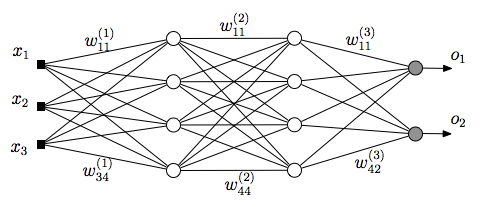
\includegraphics[scale=0.5]{img/MLP}
    \caption{Paveikslėlio pavyzdys}
    \label{img:mlp}
\end{figure}


\section{Eksperimentinio palyginimo rezultatai}
% tablesgenerator.com - converts calculators (e.g. excel) tables to LaTeX
\begin{table}[H]\footnotesize
  \centering
  \caption{Lentelės pavyzdys}
  {\begin{tabular}{|l|c|c|} \hline
    Algoritmas & $\bar{x}$ & $\sigma^{2}$ \\
    \hline
    Algoritmas A  & 1.6335    & 0.5584       \\
    Algoritmas B  & 1.7395    & 0.5647       \\
    \hline
  \end{tabular}}
  \label{tab:table example}
\end{table}

\end{document}
